\chapter{\acrlong{rc}}
\label{rc}

\section{Introduction}


% What is a rc
\gls{rc} is a bio-inspired artificial recurrent \gls{nn} which is based on the \gls{esn} paradigm introduced by Herbert Jaeger in \cite{Jaeger2004}. This computation scheme is well suited for real-time data processing and for chaotic time series prediction\cite{Jaeger2004, JaegerH.2001Tesa, Lukoeviius2012}, and achieves state of the art performances in those domains, as well as in speech recognition\cite{Verstraeten2006, NIPS2010_4056, Jaeger2007}, nonlinear channel equalisation\cite{Jaeger2004} and financial forecasting \cite{financialTimeSeries}.\\

% How is it made
A \gls{rcer} is made of a large ensemble of interconnected neurons, which are merely entities carrying an activation level. The activation level  is updated according to the connection weights of the reservoir, or \emph{synaptic matrix} as it is referred to in the field of neural networks, and with a nonlinear function, called the \textit{activation function}. The nonlinear character is one of the main features making neural networks so powerful. Moreover, with a proper activation function, one can reach a saturation state, which mimics the behaviour of biological neurons. This is traditionally achieved using the \textit{sigmoid} function. Those principles are introduced in \cite[p.227-228]{bishop2006pattern} and in \cite[p.727-728]{russell2010artificial}.\\

\begin{figure}[h]
	\centering
	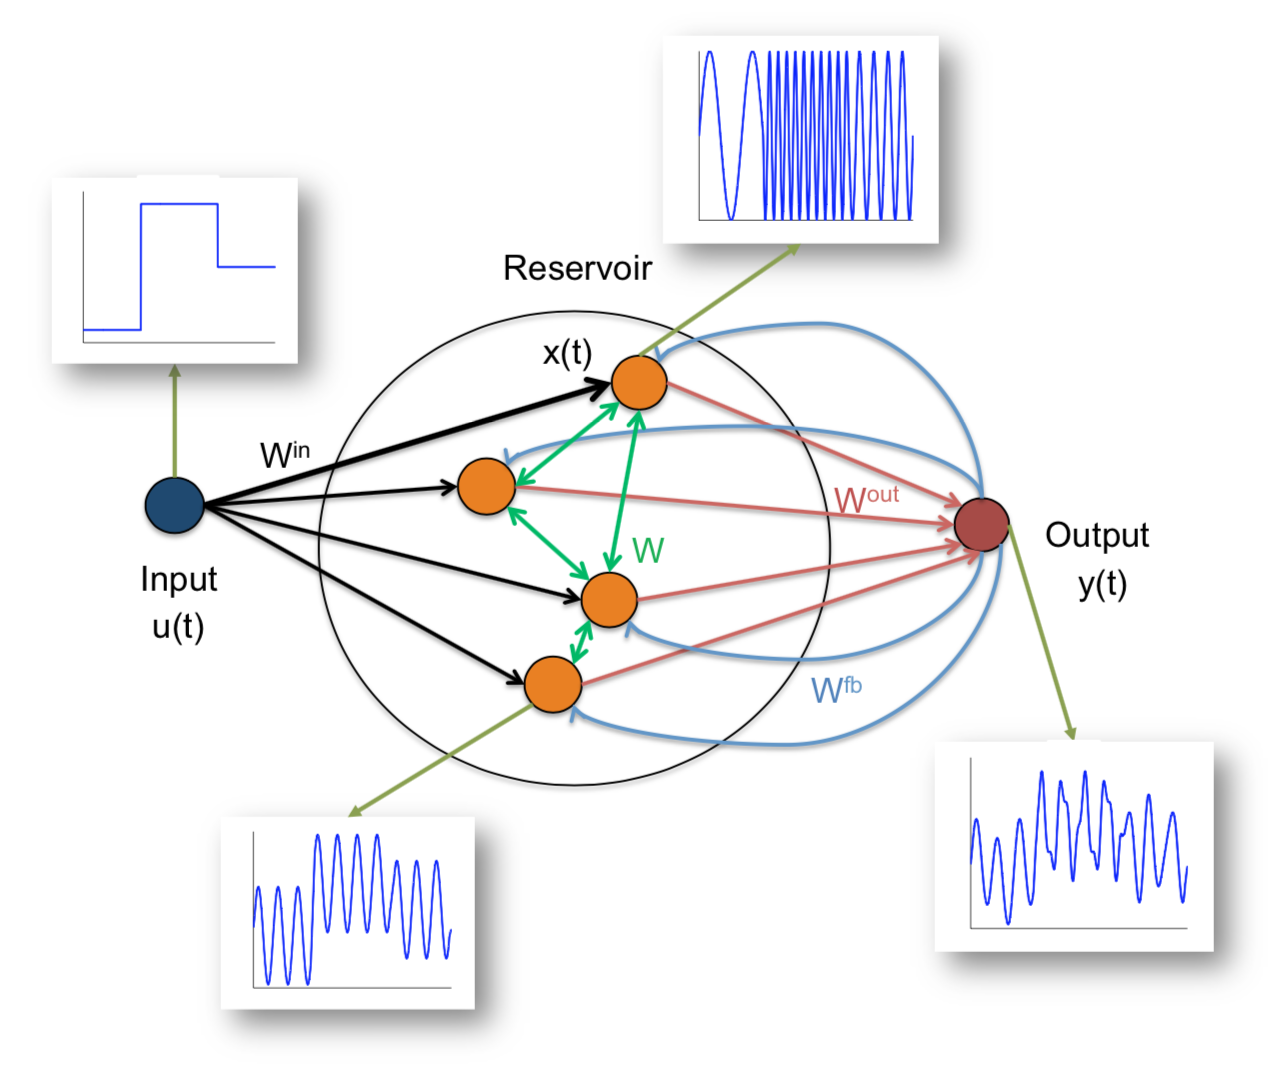
\includegraphics[width=.55\textwidth]{rc_principle.png}
	\caption{Principle scheme of a \acrshort{rcer} \cite{financialTimeSeries}}
	\label{rc_principle}
\end{figure}

% Principle of rc
The activation level of the neurons making up the reservoir characterise its state, which is a time-dependent object. The neurons are interconnected in such a way that they influence the dynamic of each other, leading to a complicated evolution of the state of the reservoir. What a first glance may seem to be a mathematical nightmare turns out to be the main advantage of \gls{rc}. Indeed, by making the connection matrix as messy as possible, \textit{i.e.} by using randomness, breaking symmetries,... one notices that the effect of such a reservoir, when being fed a time-dependent signal into the input neurons, is to map it to a higher-dimensional functional space	. \gls{rcer} reach their best performance when they are used in the echo state. This is a regime where the transients caused by the inputs are neither amplified nor damped, somehow providing a memory to the reservoir. The output of a \gls{rcer} is obtained by adequately combining the activation state of each neurons. \cite{Goudarzi2014ACS} gives a good intuitive overview of the \gls{rc} paradigm. The concepts introduced in this paragraph are illustrated at Figure \ref{rc_principle}.\\

% ML
\gls{rcer} only need the output weights to tuned through \gls{ml}, whereas other schemes of \gls{nn} usually require every weights to be adapted during training. They not only have the advantage to be computationally lighter, but they are also easier to practically implement and analyse theoretically.
